\documentclass{winnower}
\usepackage{indentfirst}
\usepackage{graphicx}
\usepackage{caption}
\usepackage{subfigure}
\usepackage{xcolor}
\usepackage{float}
\usepackage[section]{placeins}
\usepackage{multirow}
\usepackage{booktabs}
\setlength{\belowcaptionskip}{-0.5cm}

\begin{document}

\title{Homework4 report}

\author{Haoyu Guan}

\affil[1]{Questrom School of Business, Boston University}







\date{2020.02.11}

\maketitle




%-------------------------------------------------%
\section{Covariance Matrix Decomposition}
%-------------------------------------------------%


\indent Download historical data from your favorite source for 5 years and at least 100 companies or ETFs. In this problem we will
look at the covariance matrix for these assets and its properties

\vspace{12 pt}


\textbf{1. Clean the data so that your input pricing matrix is as full as possible. Fill in any
gaps using a reasonable method of your choice. Explain why you chose that particular
method.}

I choose 106 stocks from 2015 to 2020 as my data. And we cleaned the data already.
\\

\textbf{2. Generate a sequence of daily returns for each asset for each date}

\begin{figure*}[!h]
\begin{center}
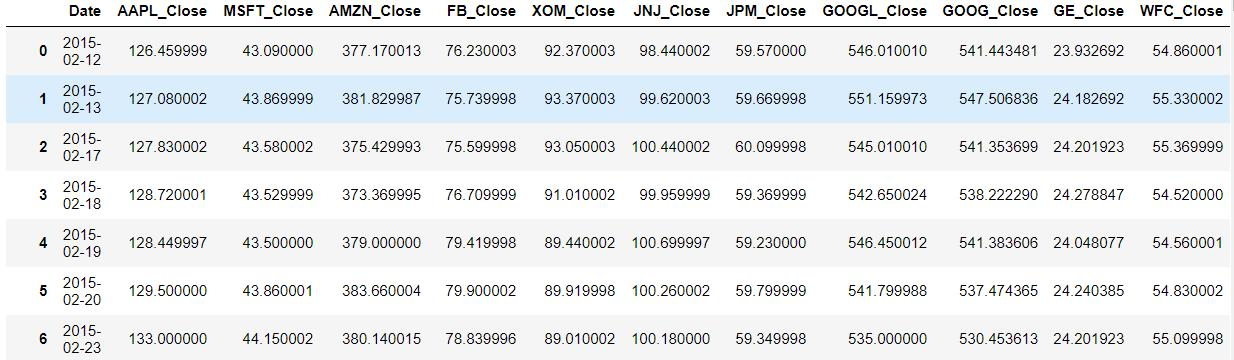
\includegraphics[scale=0.6]{1_1.jpg}
\caption
{daily return}
\label{fig:f1}
\end{center}
\end{figure*}

\newpage

\textbf{3. Calculate the covariance matrix of daily returns and perform an eigenvalue decomposition on the matrix. How many positive eigenvalues are there? How many were negative? If any are negative, what happened?}

\begin{figure*}[!h]
\begin{center}
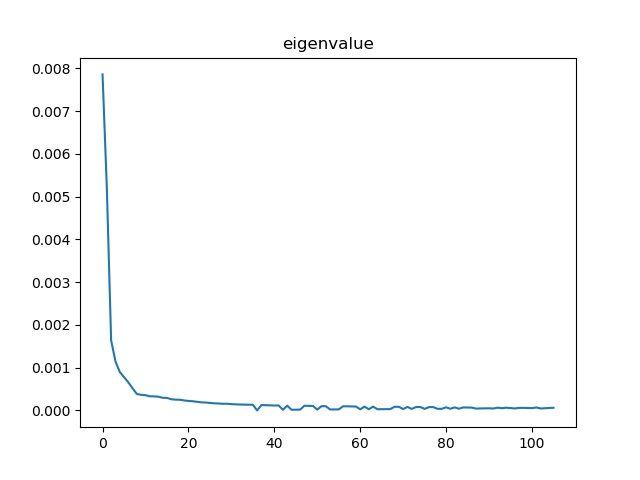
\includegraphics[scale=0.5]{1_2.jpg}
\caption
{eigenvalue}
\label{fig:f1}
\end{center}
\end{figure*}

All of the eigenvalue is positive.
\\


\textbf{4. How many eigenvalues are required to account for 50\% of the variance? How about 90\%? Does this make sense to you?}

By the calculating, 4 eigenvalues account for 50\%. And 57 eigenvalues account for 90\%
\\

\textbf{5. Using the number of eigenvalues in the 90\% threshold above, create a return stream that represents the residual return after the principal components that correspond to these eigenvalues have been removed. Plot this return stream and comment on its properties.}


\begin{figure*}[!h]
\begin{center}
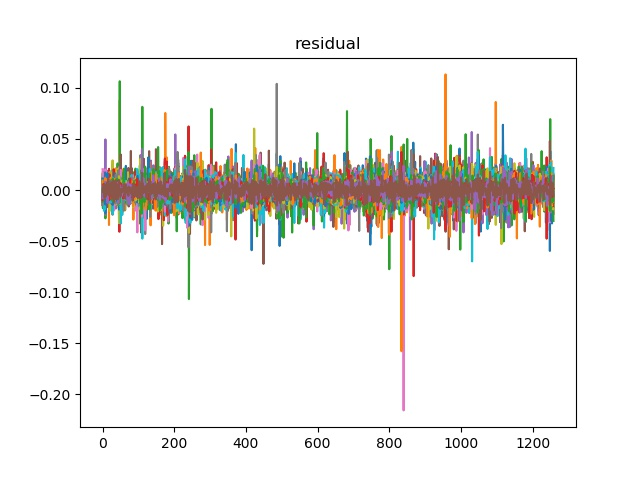
\includegraphics[scale=0.5]{1_3.jpg}
\caption
{residual}
\label{fig:f1}
\end{center}
\end{figure*}


\newpage

\section{ Portfolio Construction}

\indent In Lecture 7, we defined a Lagrangian for portfolio with constraints in matrix form by

$$L(\omega,\lambda)=<R,\omega>-a<\omega,C\omega>-<\lambda,G\omega-c>$$

\textbf{1. Form the matrix G by imposing the budget constraint, which is $<1,\omega>=1$, and another constraint that allocates 10\% of the portfolio to the first 17 securities (to simulate sector allocation). Using $C$ from Problem 1, use your favorite method and the software package of your choice to invert $GC^{-1}G^T$ in a nice, stable way. (Hint: consider my favorite method).}
\\

This is G

\begin{figure*}[!h]
\begin{center}
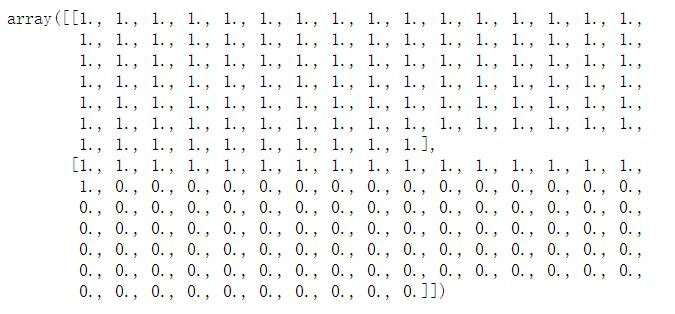
\includegraphics[scale=0.8]{1_4.jpg}
\caption
{G}
\label{fig:f1}
\end{center}
\end{figure*}

\textbf{2. What does the resulting portfolio look like? Would it be acceptable to most mutual funds? If not, what would you to do to fix that?}
\\

This is the weight of 106 stocks of my portfolio.


\begin{figure*}[!h]
\begin{center}
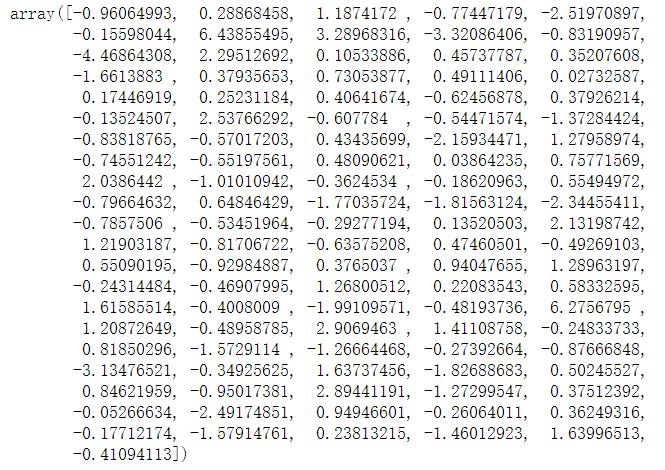
\includegraphics[scale=0.6]{1_5.jpg}
\caption
{weight}
\label{fig:f1}
\end{center}
\end{figure*}


I think this it not acceptable enough. Because we long about half of the stocks and short the other half. This portfolio may not be accepted by mutual funds because they do not usually short stock.






















\end{document}
